\documentclass[12pt]{article}
\usepackage[a4paper, margin=1in, headheight=14pt]{geometry}
\usepackage[utf8]{inputenc}
\usepackage[spanish]{babel}
\usepackage{tabularx}
\usepackage{graphicx}
\usepackage{float}
\usepackage{setspace}
\usepackage{anyfontsize}
\usepackage[toc,page]{appendix} % Remove toc,page to render wo appendix
\usepackage{hyperref}
\usepackage[table]{xcolor}
\usepackage{fancyhdr}
\usepackage{nameref}
\usepackage{datetime}
\usepackage{tikz}
\usepackage[11pt]{moresize}
\usepackage{enumerate}
\usepackage{etoolbox}


\usetikzlibrary{calc}
\newcommand\HRule{\rule{\textwidth}{1pt}}


\pagestyle{fancy}
\fancyhf{}
\fancyhead[LE,RO]{Grupo 4}
\fancyhead[RE,LO]{\nombredelproyecto}
\fancyfoot[CE,CO]{\leftmark}
\fancyfoot[LE,RO]{\thepage}

\renewcommand{\headrulewidth}{2pt}
\renewcommand{\footrulewidth}{1pt}



\newcommand{\nombredelproyecto}{\textbf{Diagrama de secuencia y de clases GUI}}
\setcounter{secnumdepth}{4}
\makeatletter
\renewcommand{\paragraph}{\@startsection{paragraph}{4}{0ex}%
    {-3.25ex plus -1ex minus -0.2ex}%
    {1.5ex plus 0.2ex}%
    {\normalfont\normalsize\bfseries}}
\makeatother

\title{\nombredelproyecto} 
\author{Jesús Abajo Magro \\
Alejandro Díaz Blázquez \\
Javier Fernández Gamo \\
Andrés Galbán Méndez \\
Alejandro Gómez Molano \\
Jaime Millán Ibáñez Archilla \\
Rodrigo Sosa Saez \\
Alejandro Barrachina Argudo}


\date{\today}

\begin{document}
\begin{titlepage}


    \makeatletter
    \centering
    \vspace*{6\baselineskip}

    %------------------------------------------------
    %	Title
    %------------------------------------------------


    {\huge \underbar{\nombredelproyecto}\par} % Title

    %------------------------------------------------
    %	Subtitle
    %------------------------------------------------

    Ingeniería del software\\
    Ingeniería informática e ingeniería de computadores

    \vspace*{3\baselineskip} % Whitespace under the subtitle


    \begin{figure}[H]
        \centering
        
\includegraphics[width=0.5\textwidth]{images/Banqueo.png}
    \end{figure}
    %------------------------------------------------
    %	Editor(s)
    %------------------------------------------------


    \vspace{0.75\baselineskip} % Whitespace before the editors
    \begin{flushright}
        \small\@author\\ % Editor list
    \end{flushright}


    \vspace{0.5\baselineskip} % Whitespace below the editor list


    \vfill % Whitespace between editor names and publisher logo

    \vspace{0.3\baselineskip} % Whitespace under the publisher logo

    \today % Publication year
    \makeatother
\end{titlepage}

\tableofcontents
\newpage
\section*{Introducción} %INTRODUCCION
En este documento se mostrarán los diagramas de clases, para mostrar las variables y métodos internos que tienen y utilizan los diferentes componentes, y los diagramas de componentes, para mostrar las partes internas de nuestro proyecto, los conectores y los puertos que implementan cada componente.

\section{Diagrama de componentes} %DIAGRAMA DE COMPONENTES
Usamos un diagrama de componentes para mostrar las partes internas y los conectores de nuestros componentes
\begin{figure}[H]
    \centering
    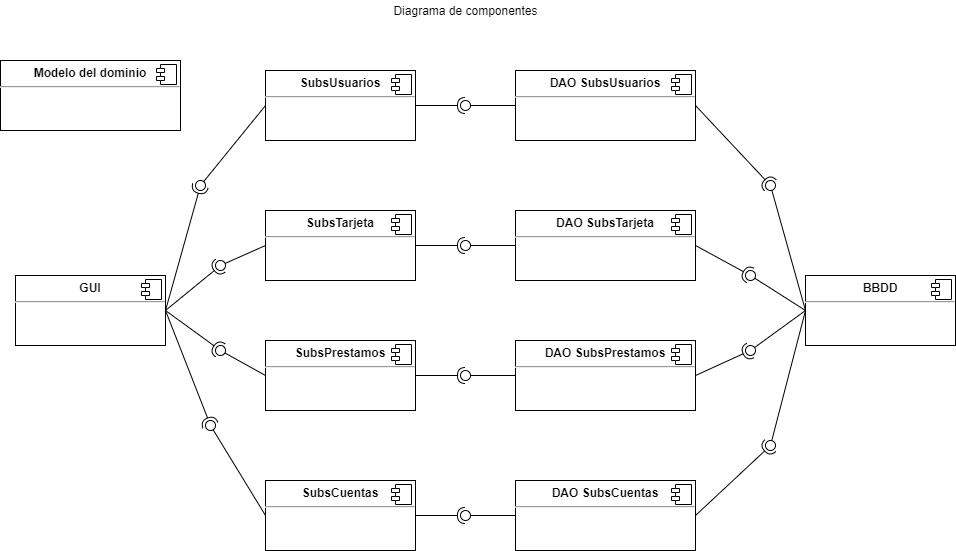
\includegraphics[width=0.8\textwidth]{images/DiagramaDeComponentes.png}
\end{figure}

\newpage
\section{Diagrama de clases para el modelo del dominio}
Usamos un diagrama de clases para mostrar el conjunto de nuestras clases,interfaces y sus relaciones
\begin{figure}[H]
    \centering
    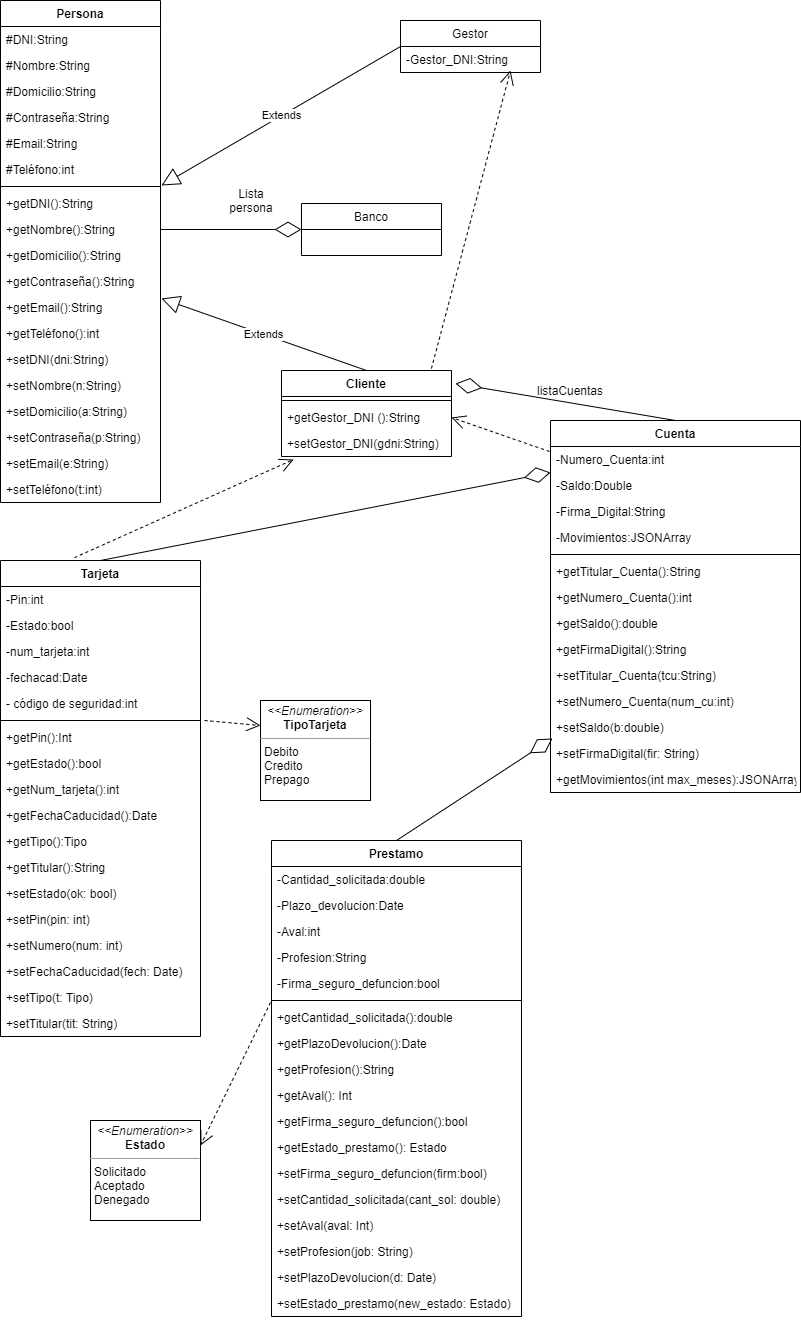
\includegraphics[width=0.8\textwidth]{images/Diagrama_de_clases.png}
\end{figure}

\newpage
\section{Diagrama de clases para la lógica del negocio de cada subsistema}
\subsection{Subsistema de cuentas}
\begin{figure}[H]
    \centering
    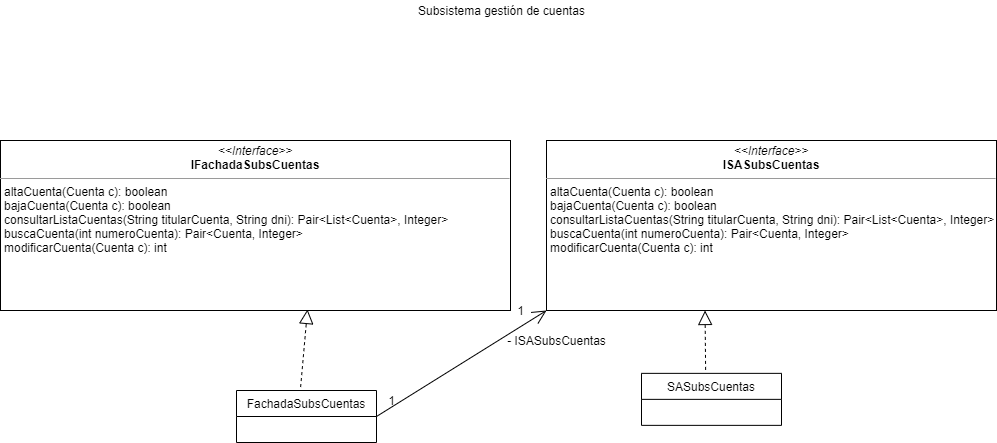
\includegraphics[width=0.8\textwidth]{images/SubsCuentas.png}
\end{figure}
\subsection{Subsistema de préstamos}
\begin{figure}[H]
    \centering
    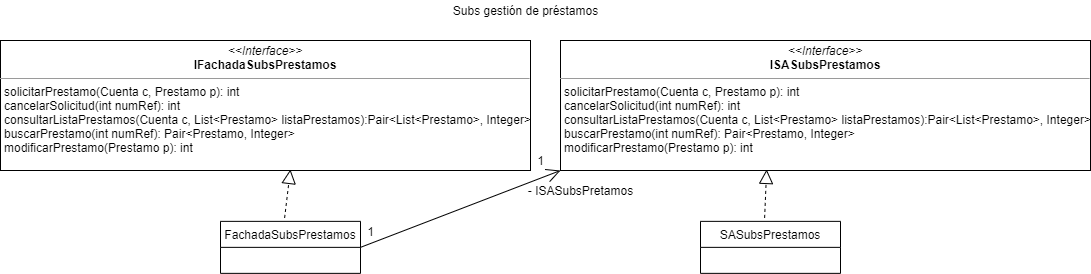
\includegraphics[width=0.8\textwidth]{images/SubsPrestamos.png}
\end{figure}
\subsection{Subsistema de tarjetas}
\begin{figure}[H]
    \centering
    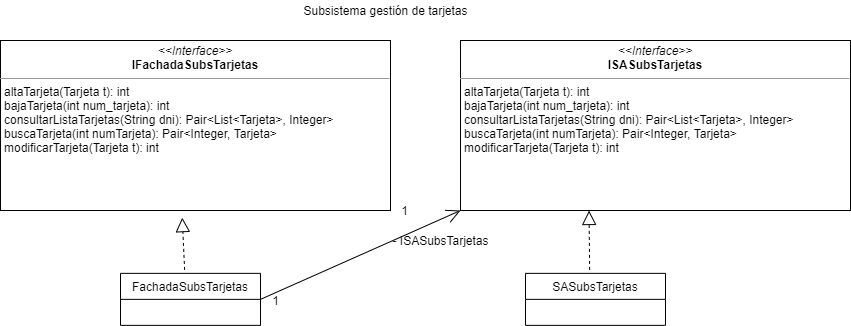
\includegraphics[width=0.8\textwidth]{images/SubsTarjeta.png}
\end{figure}
\subsection{Subsistema de usuarios}
\begin{figure}[H]
    \centering
    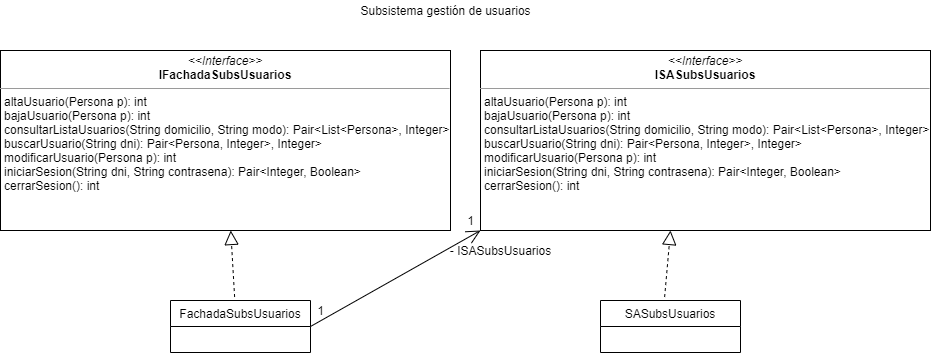
\includegraphics[width=0.8\textwidth]{images/SubsUsuarios.png}
\end{figure}

\newpage
\section{Diagrama de clases para la integración con los datos de cada subsistema}
\subsection{DAO de cuentas}
\begin{figure}[H]
    \centering
    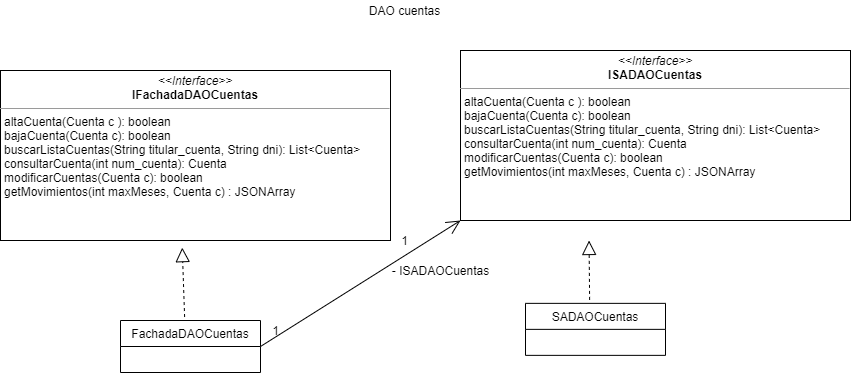
\includegraphics[width=0.8\textwidth]{images/DAOCuentas.png}
\end{figure}
\subsection{DAO de préstamos}
\begin{figure}[H]
    \centering
    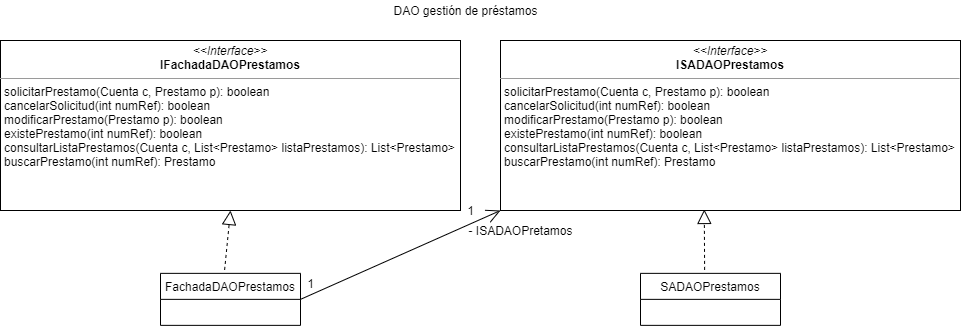
\includegraphics[width=0.8\textwidth]{images/DAOPrestamos.png}
\end{figure}
\subsection{DAO de tarjetas}
\begin{figure}[H]
    \centering
    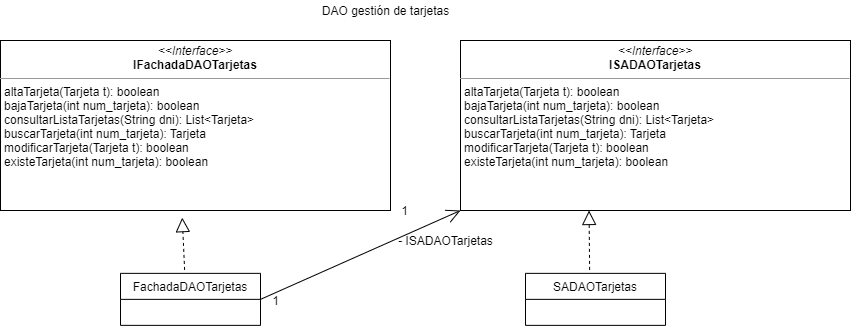
\includegraphics[width=0.8\textwidth]{images/DAOTarjeta.png}
\end{figure}
\subsection{DAO de usuarios}
\begin{figure}[H]
    \centering
    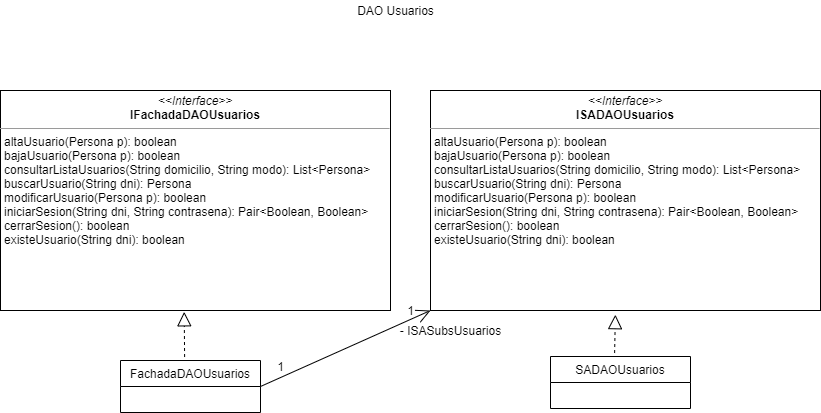
\includegraphics[width=0.8\textwidth]{images/DAOUsuarios.png}
\end{figure}
\end{document}
